\documentclass[12pt,a4paper]{article}
\usepackage[utf8]{inputenc}
\usepackage[left=20mm,top=20mm,bottom=30mm]{geometry}
\usepackage{graphicx}

\begin{document}
\title{SkyHiGH Feide}
\author{Fredrik Magnussen, Håkon Tvedt og Morten Hanssen Singstad}
\maketitle 
\begin{center}
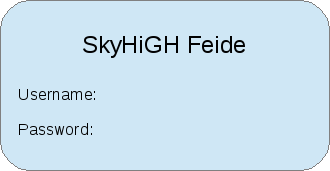
\includegraphics[scale=1]{frontpageimage.png}
\end{center}

\newpage
\tableofcontents


\newpage
\section{Forord}
Noe som fanget opp oppmerksomheten våres fra starten av, var utstyret vi skulle få sette opp og leke med. Det er ikke så mange bacheloroppgaver som passet godt for nettverksdriftere i år, derfor er denne oppgaven ekstra attraktiv, siden den er veldig relevant i henhold til driftstudie vi går. SkyHiGH Feide-oppgaven er etterfølger de tidligere SkyHiGH-oppgavene. Det som vi synes er spennende ved dette prosjektet, er at når vi er ferdig, så skal dette server-racket være oppe å kjøre og bli brukt. Den skal være høgskolens egen vm-server. Det er noe vi synes er veldig spennende.

\section{Insperation}
Let's see what happens when i do this.

\newpage
\section{Innledning}
\subsection{Bakgrunn}

\newpage
\section{Løpende dialog med arbeidsgiver Erik Hjelmås}
\subsection{Dialog med Erik Hjelmås 15-01/13}
Vi diskuterte med arbeidsgiver for å se om vi kunne få mer ressurser. Dette angående for å få server for installering av software og oppsett av Openstack på serverne i racket til SkyHiGH. Resultatet var at vi kom fram til at vi skulle bruke en av Compute nodene til å ha denne løsning i tillegg til at det skulle være en Compute node. \newline \newline

Vi diskuterte også automatisering av installasjon for hele racket. Vi hadde lest om FAI for å scripte installasjonen. Ble med dette satt på å bruke PreSeeding av kunden istedet. Grunnen til dette var kompleksiteten ved å bruke FAI, mye unødvendig og tidkrevende scripting. PreSeeding kan tidlig avbryte installasjonen for hente en preseedfil gjennom en URL for en nesten fullt ut automatisert installasjon uten å måtte svare på spørsmål om oppsett under UBUNTU 12.10 Server installeringen. Det er også muligheter for å kunne installere funksjoner som ikke er tilgjengelig i en normal installasjon. (Informasjon hentet fra [1,2]Referanser.) \newline \newline

Diskuterte også løsning på at det kunne være kjekt å kunne ha muligheten til å installere kun ved å gjøre en boot fra en USB-pinne. Det vil vi også se nærmere på om kan bli aktuelt.
\newline \newline

\newpage
\section{Dagslogg}
\subsection{15-01/13}
Timer: \newline
Fredrik 	6 t \newline
Håkon 		6 t \newline
Morten 	8 t \newline
\newline
Lest bacheloroppgaven til SkyHiGH Adm gruppa for å forstå hvordan vi skal bruke Adm sine konfigurasjoner og oppsett i Openstack. Undersøkt måter for automatisert installering av Ubuntu 12.10 Server. Sett på FAI og PreSeed og diskutert med arbeidsgiver Erik Hjelmås og funnet ut at vi går videre med PreSeed-løsningen. Installert en VM med Ubuntu 12.10 og installert controller noden ved hjelp av “install guide” fra Openstack for testing.\newline
\newline
Lest om Feide for å forstå det og skjønne hvordan vi skal klare å implementere dette inn i Openstack. Lest om Openstack for videre forståelse av hvordan det fungerer og for hvor og hvordan vi skal installere de forskjellige software-ene som skal brukes for å få et fungerende skyløsningssystem.\newline
\newline
Laget første utkast av hvordan arkitekturen skal være i racket med serverne. Hvilke software som skal til hvilke noder og hvor mange vi skal ha med de forskjellige nodene. Skrevet deler av forprosjekt og prosjektplan. Fått fungerende repository for alle medlemmene til gruppen for filene vi skriver på og oppdaterer. Laget grupperettledninger for hvordan vi skal skrive og oppdatere dokumentene uten at det skal bli tap av data.\newline
\newline
Snakket med arbeidsgiver angående videre fremgang av strøm og internett-tilgang til serverrommet og fått statusen i henhold til dette. Elektriker har vært på befaring og skal komme tilbud raskest mulig. Diskutert med arbeidsgiver angående hvordan vi skal ha en vedlikeholdsprosess på SkyHiGH.\newline
\newline
\end{document}